\documentclass[a4paper,10pt,twocolumn]{ltjarticle}
\usepackage{kaitoushu}

\pgfplotsset{
  myaxis/.style={
    axis lines=middle,
    xlabel={$x$}, ylabel={$y$},
    every axis x label/.style={at={(ticklabel* cs:1)},anchor=west},
    every axis y label/.style={at={(ticklabel* cs:1)},anchor=south},
    tick label style={font=\scriptsize},
    label style={font=\small},
    width=5.5cm, height=5cm,
    grid=none,
    samples=200,
  }
}

\begin{document}

\problemrange{5章：三角関数 — 練習問題2・A (p.156)}

\mondai{1}{次の値を求めよ．}
\kotae{
$360°$（または $2\pi$）の整数倍を加減して，扱いやすい角に直す．

\textbf{(1)} $\sin134°=\sin(180°-46°)=\sin46°=0.7193$

\textbf{(2)} $\cos(-460°)=\cos460°=\cos(460°-360°)=\cos100°$

$=\cos(180°-80°)=-\cos80°=-0.1736$

\textbf{(3)} $\tan760°=\tan(760°-720°)=\tan40°=0.8391$

\textbf{(4)} $\sin\!\left(-\dfrac{13}{3}\pi\right)=-\sin\dfrac{13}{3}\pi$

$\dfrac{13}{3}\pi-4\pi=\dfrac{13\pi-12\pi}{3}=\dfrac{\pi}{3}$ だから

$=-\sin\dfrac{\pi}{3}=-\dfrac{\sqrt{3}}{2}$

\textbf{(5)} $\dfrac{19}{6}\pi-2\pi=\dfrac{19\pi-12\pi}{6}=\dfrac{7}{6}\pi$ だから

$\cos\dfrac{19}{6}\pi=\cos\dfrac{7}{6}\pi=-\cos\dfrac{\pi}{6}=-\dfrac{\sqrt{3}}{2}$

\textbf{(6)} $\dfrac{13}{4}\pi-2\pi=\dfrac{13\pi-8\pi}{4}=\dfrac{5}{4}\pi$ だから

$\tan\dfrac{13}{4}\pi=\tan\dfrac{5}{4}\pi=\tan\dfrac{\pi}{4}=1$

（$\tan$ の周期は $\pi$ なので $\dfrac{5}{4}\pi-\pi=\dfrac{\pi}{4}$ としてもよい．）
}

\mondai{2}{$\theta$ が第4象限の角で，$\cos\theta=\dfrac{12}{13}$ のとき，$\sin\theta$，$\tan\theta$ の値を求めよ．}
\kotae{
$\sin^{2}\theta+\cos^{2}\theta=1$ より

$\sin^{2}\theta=1-\dfrac{144}{169}=\dfrac{25}{169}$

$\theta$ は第4象限の角だから $\sin\theta<0$．

$\sin\theta=-\dfrac{5}{13}$

$\tan\theta=\dfrac{\sin\theta}{\cos\theta}
=\dfrac{-5/13}{12/13}=-\dfrac{5}{12}$
}

\mondai{3}{$\tan\theta=2$ のとき，$\sin\theta$，$\cos\theta$ の値を求めよ．}
\kotae{
$1+\tan^{2}\theta=\dfrac{1}{\cos^{2}\theta}$ を使う．

$1+2^{2}=\dfrac{1}{\cos^{2}\theta}$，$\cos^{2}\theta=\dfrac{1}{5}$

$\cos\theta=\pm\dfrac{1}{\sqrt{5}}=\pm\dfrac{\sqrt{5}}{5}$

$\sin\theta=\tan\theta\cdot\cos\theta=2\cos\theta$ だから

$\sin\theta=\pm\dfrac{2}{\sqrt{5}}=\pm\dfrac{2\sqrt{5}}{5}$

$\therefore \sin\theta=\pm\dfrac{2\sqrt{5}}{5},\;\cos\theta=\pm\dfrac{\sqrt{5}}{5}$（複号同順）

$\tan\theta=2>0$ なので $\theta$ は第1象限か第3象限の角であり，
第1象限なら上の符号（ともに正），第3象限なら下の符号（ともに負）をとる．
}

\mondai{4}{次の等式を証明せよ．}
\kotae{
\textbf{(1)} $(1+\sin\theta+\cos\theta)(1+\sin\theta-\cos\theta)=2(1+\sin\theta)\sin\theta$

$1+\sin\theta$ をひとまとまりとみて，和と差の積の形にする．

左辺 $=\{(1+\sin\theta)+\cos\theta\}\{(1+\sin\theta)-\cos\theta\}$

$=(1+\sin\theta)^{2}-\cos^{2}\theta$

$=1+2\sin\theta+\sin^{2}\theta-(1-\sin^{2}\theta)$

$=2\sin\theta+2\sin^{2}\theta=2\sin\theta(1+\sin\theta)=$ 右辺 \qed

\medskip
\textbf{(2)} $\dfrac{\cos\theta}{1-\sin\theta}-\dfrac{\cos\theta}{1+\sin\theta}=2\tan\theta$

左辺を通分する．

左辺 $=\dfrac{\cos\theta(1+\sin\theta)-\cos\theta(1-\sin\theta)}{(1-\sin\theta)(1+\sin\theta)}$

$=\dfrac{2\sin\theta\cos\theta}{1-\sin^{2}\theta}
=\dfrac{2\sin\theta\cos\theta}{\cos^{2}\theta}$

$=\dfrac{2\sin\theta}{\cos\theta}=2\tan\theta=$ 右辺 \qed

\medskip
\textbf{(3)} $\dfrac{\cos^{2}\theta-\sin^{2}\theta}{1+2\sin\theta\cos\theta}=\dfrac{1-\tan\theta}{1+\tan\theta}$

分母の $1$ を $\sin^{2}\theta+\cos^{2}\theta$ に置きかえるのがポイント．

分子 $=(\cos\theta+\sin\theta)(\cos\theta-\sin\theta)$

分母 $=\sin^{2}\theta+\cos^{2}\theta+2\sin\theta\cos\theta=(\sin\theta+\cos\theta)^{2}$

よって

左辺 $=\dfrac{(\cos\theta+\sin\theta)(\cos\theta-\sin\theta)}{(\cos\theta+\sin\theta)^{2}}
=\dfrac{\cos\theta-\sin\theta}{\cos\theta+\sin\theta}$

分子・分母を $\cos\theta$ で割って

$=\dfrac{1-\tan\theta}{1+\tan\theta}=$ 右辺 \qed
}

\mondai{5}{次の関数の周期を求め，グラフをかけ．}
\kotae{
$y=\sin kx$，$y=\cos kx$ の周期は $\dfrac{2\pi}{|k|}$，
$y=\tan kx$ の周期は $\dfrac{\pi}{|k|}$．

\textbf{(1)} $y=-2\sin x$\quad 周期 $2\pi$，振幅 $2$

$y=2\sin x$ を $x$ 軸に関して折り返したグラフ．

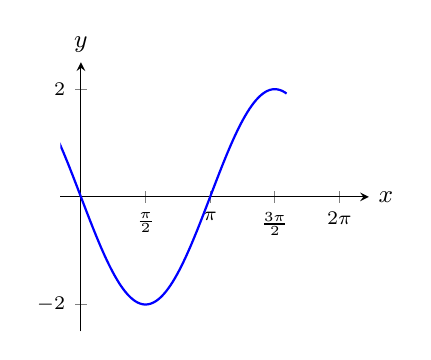
\begin{tikzpicture}
\begin{axis}[myaxis, xmin=-0.5,xmax=7,ymin=-2.5,ymax=2.5,
  xtick={1.5708,3.1416,4.7124,6.2832},
  xticklabels={$\frac{\pi}{2}$,$\pi$,$\frac{3\pi}{2}$,$2\pi$}]
\addplot[thick,blue]{-2*sin(deg(x))};
\end{axis}
\end{tikzpicture}

\textbf{(2)} $y=\dfrac{1}{2}\tan x$\quad 周期 $\pi$

漸近線は $x=\dfrac{\pi}{2}$，$x=\dfrac{3}{2}\pi$，\dots

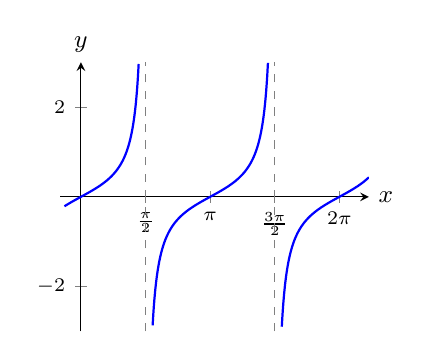
\begin{tikzpicture}
\begin{axis}[myaxis, xmin=-0.5,xmax=7,ymin=-3,ymax=3,
  xtick={1.5708,3.1416,4.7124,6.2832},
  xticklabels={$\frac{\pi}{2}$,$\pi$,$\frac{3\pi}{2}$,$2\pi$},
  restrict y to domain=-3:3]
\addplot[thick,blue,domain=-0.4:1.45]{0.5*tan(deg(x))};
\addplot[thick,blue,domain=1.70:4.59]{0.5*tan(deg(x))};
\addplot[thick,blue,domain=4.84:7]{0.5*tan(deg(x))};
\addplot[dashed,gray]coordinates{(1.5708,-3)(1.5708,3)};
\addplot[dashed,gray]coordinates{(4.7124,-3)(4.7124,3)};
\end{axis}
\end{tikzpicture}

\textbf{(3)} $y=\cos\!\left(x-\dfrac{\pi}{2}\right)$\quad 周期 $2\pi$

$y=\cos x$ を $x$ 方向に $\dfrac{\pi}{2}$ 平行移動したもので，$y=\sin x$ と一致する．

\begin{tikzpicture}
\begin{axis}[myaxis, xmin=-0.5,xmax=7,ymin=-1.5,ymax=1.5,
  xtick={1.5708,3.1416,4.7124,6.2832},
  xticklabels={$\frac{\pi}{2}$,$\pi$,$\frac{3\pi}{2}$,$2\pi$}]
\addplot[thick,blue]{cos(deg(x-1.5708))};
\end{axis}
\end{tikzpicture}

\textbf{(4)} $y=\sin\dfrac{x}{2}$\quad 周期 $\dfrac{2\pi}{1/2}=4\pi$

\begin{tikzpicture}
\begin{axis}[myaxis, xmin=-0.5,xmax=13,ymin=-1.5,ymax=1.5,
  xtick={3.1416,6.2832,9.4248,12.5664},
  xticklabels={$\pi$,$2\pi$,$3\pi$,$4\pi$},
  width=6.5cm]
\addplot[thick,blue]{sin(deg(x/2))};
\end{axis}
\end{tikzpicture}
}

\mondai{6}{次の方程式を解け．ただし $0\leqq x<2\pi$ とする．}
\kotae{
単位円をかいて，条件を満たす角をすべて拾う．

\textbf{(1)} $\sin x=-\dfrac{\sqrt{3}}{2}$

$\sin$ が負なので第3・第4象限．基準となる角は $\dfrac{\pi}{3}$．

$\therefore x=\pi+\dfrac{\pi}{3},\;2\pi-\dfrac{\pi}{3}
=\dfrac{4}{3}\pi,\;\dfrac{5}{3}\pi$

\textbf{(2)} $\cos x=\dfrac{1}{\sqrt{2}}=\dfrac{\sqrt{2}}{2}$

$\cos$ が正なので第1・第4象限．基準となる角は $\dfrac{\pi}{4}$．

$\therefore x=\dfrac{\pi}{4},\;\dfrac{7}{4}\pi$

\textbf{(3)} $\sqrt{3}\tan x=1$，すなわち $\tan x=\dfrac{1}{\sqrt{3}}$

$\tan$ の周期は $\pi$ なので，$0\leqq x<2\pi$ には解が2個ある．

$\therefore x=\dfrac{\pi}{6},\;\dfrac{\pi}{6}+\pi=\dfrac{7}{6}\pi$
}

\mondai{7}{次の不等式を解け．ただし $0\leqq x<2\pi$ とする．}
\kotae{
まず等号が成り立つ角を求め，単位円で範囲を読み取る．

\textbf{(1)} $2\sin x-1>0$，すなわち $\sin x>\dfrac{1}{2}$

$\sin x=\dfrac{1}{2}$ となるのは $x=\dfrac{\pi}{6},\;\dfrac{5}{6}\pi$．

$\sin x$ がこれより大きいのはその間だから

$\therefore \dfrac{\pi}{6}<x<\dfrac{5}{6}\pi$

\textbf{(2)} $2\cos x-\sqrt{3}<0$，すなわち $\cos x<\dfrac{\sqrt{3}}{2}$

$\cos x=\dfrac{\sqrt{3}}{2}$ となるのは $x=\dfrac{\pi}{6},\;\dfrac{11}{6}\pi$．

$\cos x$ がこれより小さいのはその間だから

$\therefore \dfrac{\pi}{6}<x<\dfrac{11}{6}\pi$
}

\end{document}
